\documentclass[conference]{IEEEtran}
\IEEEoverridecommandlockouts
% The preceding line is only needed to identify funding in the first footnote. If that is unneeded, please comment it out.
\usepackage{cite}
\usepackage{amsmath,amssymb,amsfonts}
\usepackage{algorithmic}
\usepackage{graphicx}
\usepackage{textcomp}
\usepackage{xcolor}
\usepackage{caption}
\usepackage{subcaption}
\usepackage{array}

\usepackage{mathtools} 

%added by Ye
\usepackage{fontspec}

%for typing Myanmar text, you can also used with Myanmar3 font
%\newfontfamily {\padauktext}[Script=Myanmar]{Padauk}
%\newfontinstance {\padauktext}[Script=Myanmar]{Padauk}
\newfontfamily {\padauktext}[Script=Myanmar]{Padauk}
%for double quote
\newcommand{\quotes}[1]{``#1''}
%\renewcommand{\baselinestretch}{0.86}
%added by Ye

\def\BibTeX{{\rm B\kern-.05em{\sc i\kern-.025em b}\kern-.08em
    T\kern-.1667em\lower.7ex\hbox{E}\kern-.125emX}}

%\renewcommand{\baselinestretch}{0.93}
\begin{document}


\title{Word Presentation For Paraphrase Myanmar Language Using Word2vec Model}

\author{\IEEEauthorblockN{1\textsuperscript{st} Myint Myint Htay}
\IEEEauthorblockA{\textit{University of Technology(Yatanarpon Cyber City)} \\
myintmyinthtay@utycc.edu.mm}
\and
\IEEEauthorblockN{2\textsuperscript{nd} Myat Nyein Chan}
\IEEEauthorblockA{\textit{University of Technology(Yatanarpon Cyber City)} \\
myatnyeinchan@utycc.edu.mm}
\and
\IEEEauthorblockN{3\textsuperscript{rd} May Phyo Aung}
\IEEEauthorblockA{\textit{University of Technology(Yatanarpon Cyber City)} \\
mayphyoaung@utycc.edu.mm}
\and
\IEEEauthorblockN{4\textsuperscript{th} Ei Phyu Phyu Mon}
\IEEEauthorblockA{\textit{University of Technology(Yatanarpon Cyber City)} \\
eiphyuphyumon@utycc.edu.mm}
}

\maketitle

\begin{abstract}
Word2Vec methods are widely used to evaluate similarity scores and to classify text in a variety of language. Both skipgram and CBOW are also two of the most popular methods based on word2vec in state-of-art natural language processing (NLP). Skipgram works well with small amount of data and is found to represent rare words well. When we anlaysed the two experiments with large amount of data, Continuous Bag-of-Word (CBOW) was faster and got better representations for more frequent words. This paper analyses the performance of two models with similarity scores and processing time for myanmar language (Burmese).  Data are collected  in domain with respect to the travelling and daily general conversations.\end{abstract}

\begin{IEEEkeywords}
Word Embedding, Word2vec, CBOW, skipgram
\end{IEEEkeywords}

\section{Introduction}
\label{Sec:introduction}

Natural Language Processing (NLP) is the field of artificial intelligence that studies the interactions between computers and human languages, in particular how to program computers to process and analyze large amounts of natural language data. NLP is often applied for classifying text data. Text classification is the problem of assigning categories to text data according to its content. There are different techniques to extract information from raw text data and use it to train a classification model. These techniques are Bag-of-Words (used with a simple machine learning algorithm such as Tf-Idf), the popular word embedding model Word Embedding (used with a deep learning neural network such as Word2Vec), and the state-of-the art Language models (used with transfer learning from attention-based transformers such BERT) that have completely revolutionised the NLP landscape. All of these techniques, we applied this proposed system by using word embedding. There is a lot of progress  being currently made in NLP using word embedding, it is a positive trend that can be used in a very broad range of practical NLP applications such as computing the similarities between words, using as features in text classification and different natural language tasks such as sentiment analysis. Word2Vec produces a vector space, typically of several hundred dimensions, with each unique word in the corpus such that words that share common contexts in the corpus are located close to one another in the space. That can be done using 2 different approaches: starting from a single word to predict its context (skipgram) or starting from the context to predict a word (Continuous Bag-of- Words). The word embedding can be useful to predict the news category. The word vectors can be used in a neural network as weights. First, the corpus is transformed into padded sequences of word ids to get a feature matrix. Then, create an embedding matrix so that the vector of the word with id N is located at the Nth row. Finally, build a neural network with an embedding layer that weighs every word in the sequences with the corresponding vector. In this proposed paper, we analyzed the performance of skipgram and CBOW models on both small amount of training data (only 100 senteces) and large amount of training data (242,327 sentences).

\section{Related Work}\label{Sec:relatedwork}

In \cite{b1} showed that where embeddings factorise pointwise mutual information (PMI), it is paraphrasing that determines when a linear combination of embeddings equates to that of another word. They derived a probabilistically grounded definition of paraphrasing that they reinterpret as word transformation, a mathematical description of  ``w\textsubscript{x} is to w\textsubscript{y}''. From these concepts they proved that the existence of linear relationships between W2V-type embeddings that underlie the analogical phenomenon, identifying explicit error terms. \cite{b2} addressed the OOV problem for low resource SMT by paraphrasing with word embeddings and semantic lexicons. They proposed using semantic lexicons including WordNet, FrameNet, and the Paraphrase Database (PPDB) for paraphrasing. In addition, they applied a method to combine these two types of paraphrases, which achieved further improvements in SMT. OOV paraphrasing that augments the translation model for the OOV words by using the translation knowledge of their paraphrases has been proposed to address the OOV problem. In this paper, authors proposed using word embeddings and semantic lexicons for OOV paraphrasing. The lower coverage of the semantic lexicons compared to Word2vec, leading to lower OOV decreases. The combination of Word2vec and the semantic lexicons by retrofitting outperformed either method, because of the quality improvement of the word embeddings. Word2vec retrofitted by PPDB achieved the best performance. They showed that the reason for this is the higher coverage of PPDB compared to the other semantic lexicons, leading to more improvement of the word embeddings.  David Guthrie et al. \cite{b3} examined the use of skipgrams to overcome the data sparsityproblem. Data sparsity was a large problem in natural language processing that even using an extremely large corpus, NLP researchers can never accurately model all possible strings of words. They investigated skipgram modeling using one to four skips with various amount of training data and test against similar documents as well as documents generated from a machine translation system. In the paper, they also determined the amount of extra training data required to achieve skipgram coverage using standard adjacent trigram. These paper was focus to quantify the impact skipgram modeling has on the coverage of trigram in real text and compared this to coverage obtained by increasing the size of he corpus used to build a traditional language model. In this survey \cite{b4}, authors highlighted the latest studies on using the Word2vec model for sentiment analysis and its role in improving sentiment classification accuracy, and presented a literature review of several studies that used the word2vec model for sentiment analysis. According to this literature that most studies were used the two methods of word2vec: CBOW and skipgram, and compared the results from each method. skipgram is better for infrequent words than CBOW, however, CBOW is faster and works well with frequent words. Many of the studies in literature applied word2vec using tools such as word2vec tool and FastText. Text preprocessing in \cite{b5} is important part to build embedding model. This paper tries to extract the analogous words between Myanmar news articles focus on the bag of words (CBOW) model using different features vector sizes. By analyzing word embedding model are obtained the better results with high-dimensional vectors than low-dimensional vectors to cluster the words based on its relatedness. Using the concept of word embeddings is to increase the accuracy of the sentiment identification in \cite{b6}. Word2Vec is used to train for producing high-dimensional word vectors that learns the syntactic and semantic of word. The resulting word vectors train Machine Learning algorithms in the form of classifiers for sentiment identification. The use of word embeddings from the collected real-world datasets improves the accuracy of sentiments classification.

\section{Word Segmentation}\label{Sec:wordsegmentation}
Word segmentation is the very important method for the text analysis level. The under resource languages such as Burmese text are not usually separate with white space between words. The white spaces are often used to distinguish sentences for easier reading. We also used word segmentation method \cite{b7} and additionally manually segmented for Burmese word segmentation process.

\section{Data Collection}\label{Sec:datacollection}
In Burmese, various words and various conversation styles for the same performance in daily conversation and travelling domain. Some of the paraphrase sentences are different only one word in that sentence and some sentences are quite different for the whole sentences. Some of the sentences are collected from social media (Facebook comments) and the comments are collected from the famous Myanmar news websites by extracting the Facepager Tool (version 4.2.7) \cite{b8}. Comments in social media are collected as needed as the sentences for our requirements in data in the range of travel domain and daily general conversations. Moreover, some are collected from the Burmese Wiktionary \cite{b9} site and extraction with Web Scraper tool. We also used travel domain data from \cite{10}. Using these words and we built more of the paraphrase sentences for our research. Based on \cite{b11} in this research, we used 242,327 total sentences to train, validate and predict results unsupervisedly. The Burmese  corpus is a UTF-8 plain text file.


\section{Methodology}\label{Sec:Methodology}

Humans have always excelled at understanding languages. It is easy for humans to understand the relationship between words but for computers, this task may not be simple. For example, humans understand the words like king and queen, man and woman, have a certain type of relation between them but a computer how to do this.

Word embedding are basically a form of word representation that bridges the human understanding of language to that of a machine. They have learned representations of text in an n-dimensional space where words that have the same meaning have a similar representation. Meaning that two similar words are represented by almost similar vectors that are very closely placed in a vector space. These are essential for solving most Natural language processing problems.

When using word embeddings, all individual words are represented as real-valued vectors in a predefined vector space. Each word is mapped to one vector and the vector values are learned in a way that resembles a neural network. As the machine learning models cannot process text, consequently, we need to figure out a way to convert these textual data into numerical data. The main target of word embedding model is to convert word to the form of numeric vectors. We need to do word embedding because many machine learning algorith ms and most of the deep learn ing architectures cannot process the raw form of strings or plain texts. There are several models to learn word embedding.  They  are count-vector, tf-idf vectorization , co-occurrence matrix and Word2Vec.

Word2vec is a method to efficiently create word embeddings by using a two-layer neural network. It was developed by Tomas Mikolov, at Google in 2013 as a response to make the neural-network-based training of the embedding more efficient and since then has become the de facto standard that is a voluntary standard, for developing pre-trained word embedding. Word2vec is a group of related models that are used to produce word embeddings. These models are shallow, two-layer neural networks that are trained to reconstruct linguistic contexts of words. Word2vec takes as its input a large corpus of text and produces a vector space, typically of several hundred dimensions, with each unique word in the corpus being assigned a corresponding vector in the space. Word vectors are positioned in the vector space such that words that share common contexts in the corpus are located close to one another in the space.

While Word2vec is not a deep neural network, it turns text into a numerical form that deep neural networks can understand. The Word2Vec objective function causes the words that have a similar context to have similar embedding. Consequentyly, in this vector space, these words are really close.

Word2vec is not a single algorithm but a combination of two techniques – CBOW and skipgram model. Both of these are shallow neural networks which map word(s) to the target variable which is also a word(s). Both of these techniques learn weights which act as word vector representations. Skip Gram works on small amount of training  data and it can represent for rare words or phrases. Continuous Bag of Words model is faster than the skip gram model and it can train on large amount of  data and it is slightly better accuracy for the frequent words.

\subsection{Continuous Bag-of-Words Model (CBOW)}

Continuous Bag-of-Words Model which predicts the middle word based on surrounding context words. The context consists of a few words before and after the current (middle) word. This architecture is called a bag-of-words model as the order of words in the context is not important. It predicts the probability of a word to occur given the words surrounding it, and can consider a single word or a group of words. But for simplicity, a single context word will be taken and try to predict a single target word. For example, we will consider that the corpus contains only one sentence, that being, `{\padauktext သူ ကျောင်း သို့ သွားသည်}' (as English: `He goes to school').
First, we convert each word into a one-hot encoding form(see Fig.~\ref{fig:cbowskipAfig}). Also, we’ll not consider all the words in the sentence but only take certain words that are in a window. For example, for a window size equal to three, we only consider three words in a sentence. The middle word is to be predicted and the surrounding two words are fed into the neural network as context. The window is then slid and the process is repeated again. Finally, after training the network repeatedly by sliding the window a shown in Fig.~\ref{fig:cbowBfig}, we get weights which we use to get the embedding as shown in Fig.~\ref{fig:cbowCfig}. 

\begin{figure}
     \centering
     \begin{subfigure}[b]{0.5\textwidth}
         \centering
         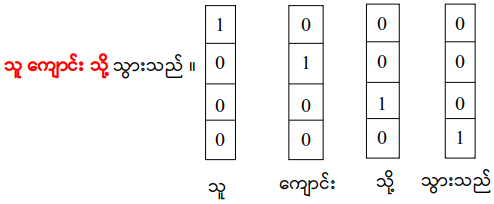
\includegraphics[width=0.5\textwidth]{./fig/cbow-skip-a.png}
  	 \caption{Convert each word into a one-hot encoding form}
         \label{fig:cbowskipAfig}
     \end{subfigure}
     \hfill
     \begin{subfigure}[b]{0.5\textwidth}
         \centering
         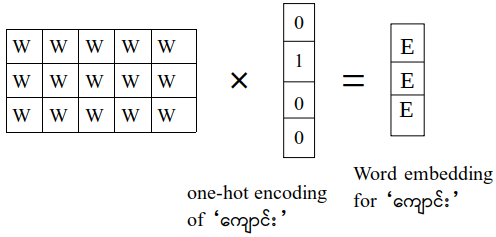
\includegraphics[width=0.5\textwidth]{./fig/cbow-b.png}
 	 \caption{Weights are used to get the embedding} 
	 \label{fig:cbowBfig}
     \end{subfigure}
     \hfill
     \begin{subfigure}[b]{0.5\textwidth}
         \centering
         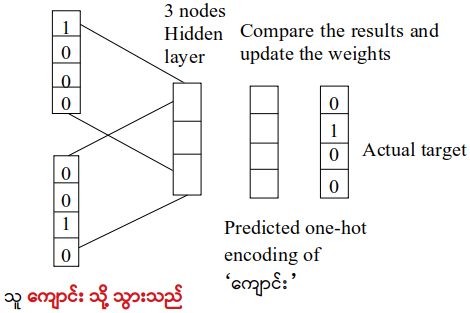
\includegraphics[width=0.5\textwidth]{./fig/cbow-c.png}
         \caption{Training the network repeatedly by sliding the window}
	 \label{fig:cbowCfig}
     \end{subfigure}
        \caption{Model architectures of CBOW}
        \label{fig:cbow}
\end{figure}

\subsection {Skipgram Model (skipgram)}
Continuous skipgram Model which predicts words within a certain range before and after the current word in the same sentence. skipgrams are a technique largely used in the field of speech processing, whereby n-grams are formed (bi-grams, trigram, etc.) but in addition to allowing adjacent sequences of words, we allow tokens to be ``skipped''. While initially applied to phonemes in human speech, the same technique can be applied to words. For example, the sentence ``I hit the tennis ball'' has three-word level trigram: ``I hit the'', ``hit the tennis'' and ``the tennis ball''. However, one might argue that an equally important trigram implied by the sentence but not normally captured in that way is ``hit the ball''. Using skipgrams allows the word ``tennis'' be skipped, enabling this trigram to be formed. skipgrams have been used many different ways in language modeling but often in conjunction with other modeling techniques or for the goal of decreasing perplexity.
An actual sentence example shows 2-skip-bigram and trigram compared to standard bi-grams and trigram consisting of adjacent words for the sentence:

“Insurgents killed in ongoing fighting.”
Bigram = {insurgents killed, killed in, in ongoing, ongoing fighting}.

2-skip-bigram = {insurgents killed, insurgents in, insurgents ongoing, killed in, killed ongoing, killed
fighting, in ongoing, in fighting, ongoing fighting}

trigram = {insurgents killed in, killed in ongoing, in ongoing fighting}.

2-skip-trigram = {insurgents killed in, insurgents killed ongoing, insurgents killed fighting, insurgents in ongoing, insurgents in fighting, insurgents ongoing fighting, killed in ongoing, killed in fighting, killed ongoing fighting, in ongoing fighting}. 

Use k-skip gram to mean k skips or less for an n word sentence.
%which can be written as:
%\begin{equation}
%\label{eq:1}
%{n}\[\sum_{i=1}^{k+1}{i-}\sum_{i=1}^{k+1}{i(i+1)}\\\text{=}\frac{(k+1)(k+2)(3n-2k-6)}{6}\\
%\text{for n>k+2}
%\end{equation}

%\begin{equation}
%\label{eq:1}
%\Hat{e}=argmax_e \mathbf {P}(e|f)
%\end{equation}
The skipgram model architecture usually tries to achieve the reverse of what the CBOW model does. It tries to predict the source context words (surrounding words) given a target word (the centre word). The working of the skipgram model is quite similar to the CBOW but there is just a difference in the architecture of its neural network and the way the weight matrix is generated as shown in the Fig.~\ref{fig:cbowskipAfig} and Fig.~\ref{fig:skipBfig}. After obtaining the weight matrix, the steps to get word embedding is same as CBOW.

\begin{figure}
     \centering
     \begin{subfigure}[b]{0.5\textwidth}
         \centering
         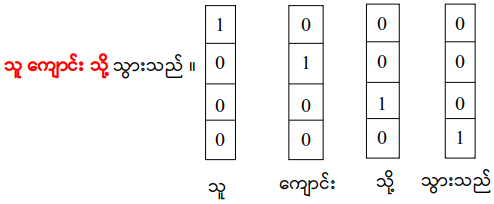
\includegraphics[width=0.5\textwidth]{./fig/cbow-skip-a.png}
  	 \caption{Convert each word into a one-hot encoding form}
         \label{fig:cbowskipAfig}
     \end{subfigure}
     \hfill
     \begin{subfigure}[b]{0.5\textwidth}
         \centering
         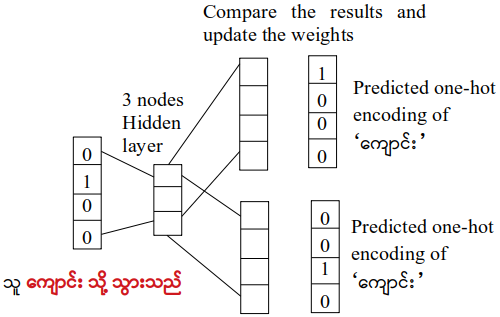
\includegraphics[width=0.5\textwidth]{./fig/skip-gram-b.png}
 	 \caption{Training the network repeatedly by sliding the window} 
	 \label{fig:skipBfig}
     \end{subfigure}
        \caption{Model architectures of skipgram}
        \label{fig:skip}
\end{figure}


\section {Experimental Setup}\label{Sec:experimentalsetup}
In this proposed paper, we applied fastText python library (fasttext 0.9.2) \cite{b12}. It is a library for efficient learning of word representations and sentence classification. fastText provides two models for computing word representations: skipgram and CBOW (`continuous-bag-of-words'). Let us illustrate this difference with an example: given the sentence 'Poets have been mysteriously silent on the subject of cheese' and the target word `silent', a skipgram model tries to predict the target using a random close-by word, like `subject' or `mysteriously'. The CBOW model takes all the words in a surrounding window, like {been, mysteriously, on, the}, and uses the sum of their vectors to predict the target. We run fastText with the default parameters, but depending on the data, these parameters may not be optimal. The most important parameters of the model are its dimension and the range of size for the subwords. The dimension (dim) controls the size of the vectors, the larger they are the more information they can capture but requires more data to be learned. But, if they are too large, they are harder and slower to train. By default, we use 100 dimensions, but any value in the 100-300 range is as popular. The subwords are all the substrings contained in a word between the minimum size (minn) and the maximal size (maxn). By default, we take all the subword between 3 and 6 characters, but other range could be more appropriate to different languages. Depending on the quantity of data you have, you may want to change the parameters of the training. The epoch parameter controls how many times the model will loop over your data. By default, we loop over the dataset 5 times. If you dataset is extremely massive, you may want to loop over it less often. Another important parameter is the learning rate -lr. The higher the learning rate is, the faster the model converge to a solution but at the risk of overfitting to the dataset. The default value is 0.05 which is a good compromise. Finally , fastText is multi-threaded and uses 12 threads by default. If you have less CPU cores (say 4), you can easily set the number of threads using the thread flag. In this experiment, we applied default parameters. In order to find nearest neighbors, we need to compute a similarity score between words. Our words are represented by continuous word vectors and we can thus apply simple similarities to them. In a similar spirit, one can play around with word analogies by applying (gensim 3.7.3) \cite{b13} to find similarity words. Gensim is a Python library for topic modelling, document indexing and similarity retrieval with large corpora. Target audience is the natural language processing (NLP) and information retrieval (IR) community.

\section {Results and Discussion}
\label{sec:ResultsandDiscussion}
At first, we experimented both skipgram and CBOW based on only training data 100 sentences. The experiment of skipgram,  we can see if our model can guess what is to `{\padauktext အဆာပြေ}', and what `{\padauktext အဆာပြေ}' is to `{\padauktext မနက်စာ}'. This can be done with the analogies functionality. It takes a word triplet (like {\padauktext မနက်စာ  ထမင်း အဆာပြေ}) and outputs the analogy as:\\

\begingroup
Query triplet (A - B + C)? {\padauktext မနက်စာ - ထမင်း + အဆာပြေ }\\
{\padauktext ချင်ရဲပြေ} 0.745777\\
{\padauktext ထမင်းအေး} 0.720301\\
{\padauktext အာသာပြေ} 0.719034\\
{\padauktext ထမင်းဟင်း} 0.714321\\
{\padauktext ထမင်းမေ့ဟင်းမေ့} 0.69706\\
{\padauktext ဆာ} 0.692757\\
{\padauktext ထမင်းရေ} 0.681634\\
{\padauktext စားနေကျ} 0.680725\\
{\padauktext အာသီသ} 0.678317\\
{\padauktext အာသာဆန္ဒ} 0.677543\\\endgroup

Our skipgram model considers that the `{\padauktext အဆာပြေ}' analogy of a `{\padauktext မနက်စာ}' is the `{\padauktext ချင်ရဲပြေ}', which seems reasonable. 

In the experiment of CBOW,  we can see if our model can guess what is to `{\padauktext အဆာပြေ}', and what `{\padauktext အဆာပြေ}' is to `{\padauktext မနက်စာ}'. This can be done with the analogies functionality. It takes a word triplet like {\padauktext မနက်စာ  ထမင်း အဆာပြေ} and outputs the analogy as:\\

\begingroup
Query triplet (A - B + C)? {\padauktext မနက်စာ - ထမင်း + အဆာပြေ }\\
{\padauktext နေ} 0.148211\\
{\padauktext ပါ} 0.142243\\
{\padauktext မယ်} 0.13875\\
{\padauktext ကြ} 0.128288\\
{\padauktext စောက်} 0.128086\\
{\padauktext ရှိ} 0.127845\\
{\padauktext ရ} 0.12631\\
{\padauktext နိုင်} 0.104394\\
{\padauktext တွေ} 0.066768\\
{\padauktext ။} 0.0393234\\\endgroup

Our CBOW model considers that the `{\padauktext အဆာပြေ}' analogy of a `{\padauktext မနက်စာ}' is the `{\padauktext နေ}', which seems not reasonable. 
Our CBOW model considers that the `{\padauktext အဆာပြေ}' analogy of a `{\padauktext မနက်စာ}' is the `{\padauktext နေ}', which seems not reasonable. 

According to the above two experiments which are based on only training data(100 sentences), we observed that the skipgram gets more closet words `{\padauktext ချင်ရဲပြေ}' with similarity score `0.745777' while the CBOW getting the closet word `{\padauktext နေ}' with similarity score '0.18086' for the input triplet `{\padauktext မနက်စာ - ထမင်း + အဆာပြေ}'. Thus, the skipgram experiment gets more reasonable outcomes with better similarity scores than the experiment of CBOW with only training data (100 sentences).

And then, we analyzed both skipgram and CBOW based on training data (242,327 sentences). The experiment of skipgram outputs the analogy as:\\

\begingroup
Query triplet (A - B + C)? {\padauktext မနက်စာ - ထမင်း + အဆာပြေ }\\
{\padauktext ထမင်းဟင်း} 0.743704\\
{\padauktext ထည့်သွင်း} 0.682644\\
{\padauktext ဒင်း} 0.67533\\
{\padauktext မကျန်မကြွင်း} 0.672617\\
{\padauktext ထမင်းရည်ပူလာလျှာလွှဲ} 0.672009\\
{\padauktext ဒံပေါက်ထမင်း} 0.657037\\
{\padauktext မဂ္ဂဇင်း} 0.657002\\
{\padauktext ဟိုသင်း} 0.648797\\
{\padauktext ထမင်းစားပြီး} 0.64839\\
{\padauktext ဧည့်မြေ} 0.647002\\\endgroup

Our skipgram model considers that the `{\padauktext အဆာပြေ}' analogy of a `{\padauktext မနက်စာ}' is the `{\padauktext ထမင်းဟင်း}'.\\

The experiment of CBOW outputs the analogy as:

\begingroup
Query triplet (A - B + C)? {\padauktext မနက်စာ - ထမင်း + အဆာပြေ }\\
{\padauktext ထမင်းဟင်း} 0.777087\\
{\padauktext လမင်း} 0.749024\\
{\padauktext အိုမင်း} 0.731996\\
{\padauktext မယ်မင်း} 0.718184\\
{\padauktext မကျန်မကြွင်း} 0.712241\\
{\padauktext မဂ္ဂဇင်း} 0.710967\\
{\padauktext စင်း} 0.708923\\
{\padauktext အခင်း} 0.708785\\
{\padauktext ဒင်း} 0.707475\\
{\padauktext မနက်လင်း} 0.70745\\\endgroup

Our CBOW model also considers that the `{\padauktext အဆာပြေ}' analogy of a `{\padauktext မနက်စာ}' is the `{\padauktext ထမင်းဟင်း}', which seems reasonable. 
According to the above two experiments which are based on training data (242,327 sentences), we observed that the CBOW outputted the closet word `{\padauktext ထမင်းဟင်း}' with similarity score `0.777087' while the skipgram also getting the same closet word `{\padauktext ထမင်းဟင်း}' with similarity score '0.743704' for the input triplet `{\padauktext မနက်စာ - ထမင်း + အဆာပြေ}'. Thus, if the training data size is cover for all testing data, the CBOW experiment gets more reasonable outcomes with better similarity scores than the experiment of skipgram. Of course the quality of the analogies depend on the dataset used to train the model and one can only hope to cover fields only in the dataset. 

Besides, we studied on the experiment of subword for both skipgram and CBOW. Using subword-level information is particularly interesting to build vectors for unknown words. For skipgram model, by using subword ({\padauktext အဆာပြေ}) information gives the following list of nearest neighbors:\\

\begingroup
Query word: {\padauktext အဆာပြေ}\\
{\padauktext အမောပြေ} 0.846186\\
{\padauktext အာသာပြေ} 0.829208\\
{\padauktext ညာပြော} 0.770294\\
{\padauktext အဆင်ပြေပြေ} 0.770002\\
{\padauktext စိမ်ပြေနပြေ} 0.756734\\
{\padauktext ဘာပြော} 0.750311\\
{\padauktext ခရာတာတာပြော} 0.744353\\
{\padauktext ဆိုကျေပြီမလား} 0.740593\\
{\padauktext ပြေစာ} 0.738888\\
{\padauktext ပြေ} 0.738307\\
\endgroup
For CBOW model, by using subword ({\padauktext အဆာပြေ}) information gives the following list of nearest neighbors:\\

\begingroup
Query word: {\padauktext အဆာပြေ}\\
{\padauktext အဆင်ပြေပြေ} 0.883487\\
{\padauktext အာသာပြေ} 0.87291\\
{\padauktext ဆင်ပြေ} 0.848755\\
{\padauktext အဆင်ပြေ} 0.823117\\
{\padauktext စိမ်ပြေနပြေ} 0.818285\\
{\padauktext အမောပြေ} 0.790669\\
{\padauktext အဆင်မပြေ} 0.790384\\
{\padauktext ဖျန်ဖြေ} 0.779151\\
{\padauktext ညာပြော} 0.768855\\
{\padauktext ခရာတာတာပြော} 0.767131\\\endgroup

Therefore, we observed that the CBOW model also outperforms than the skipgram model in sub-word experiment for Myanmar language(Burmese). Both the execution time of skipgram and CBOW are fast because the execution time of skipgram takes only 0m19.210s while the execution time of CBOW takes only 0m18.228s for all training data (242,327 sentences).

\section{Conclusion}\label{sec:Conclusion}
Performance of two word2vec models for myanmar language are evaluated in similarity scores and processing time. Data about travel domain and daily general conversations are collected from social media. For both CBOW and skipgram, sentences are evaluated with style of nearess and subword. CBOW achieved better similarity scores and faster than skipgram in the experiment of data size (242,327 sentences). But skipgram also outperforms good result in the experiment of data size only (100 sentences). Consequently, the quality of the analogies depend on the dataset used to train the model and one can only hope to cover fields only in the dataset. As our future work, the strength of CBOW and skipgram methods based on word2vec will be applied for text classification and sentiment analysis for Myanmar NLP trend.

\begin{thebibliography}{00}

\bibitem{b1} Carl Allen and Timothy Hospedales, ``Analogies Explained: Towards Understanding Word Embeddings,'' Proceedings of the 36th International Conference on Machine Learning, Long Beach, California, PMLR 97, 2019.
\bibitem{b2} Chenhui Chu and Sadao Kurohashi, ``Paraphrasing Out-of-Vocabulary Words with Word Embeddings and Semantic Lexicons for Low Resource Statistical Machine Translation''.
\bibitem{b3} David Guthrie and Ben Allison, Wei Liu, Louise Guthrie, Yorick Wilks, ``A Closer Look at skipgram Modeling,'' Research Gate, December 2014.
\bibitem{b4} Samar Al-Saqqa and Arafat Awajan, ``The Use of Word2vec Model in Sentiment Analysis: A Survey,'' Research Gate, December 2019.
\bibitem{b5} Aye Myat Mon and Khin Mar Soe, ``Clustering Analogous Words in Myanmar Language using Word Embedding Model,'' ICCA and ICFCC Conference, February 2019.
\bibitem{b6} Hay Mar Su Aung and Win Pa Pa, ``Analysis of Word Vector Representation Techniques with Machine-Learning Classifiers for Sentiment Analysis of Public Facebook Page’s Comments in Myanmar Text,'' IEEE Conference on Computer Applications (ICCA), February 2020.
\bibitem{b7}W. P. Pa, Y. K. Thu, A. Finch, and E. Sumita, ``Word boundary identification for Myanmar text using conditional random fields'', in International Conference on Genetic and Evolutionary Computing.
Springer, pp. 447–456, 2015.
\bibitem{b8}https://github.com/strohne/Facepager/releases/
\bibitem{b9}https://my.wiktionary.org/wiki/
\bibitem{10}https://raw.githubusercontent.com/ye-kyaw-thu/myPOS/master/corpus-draft-ver-1.0/mypos-dver.1.0.cword.txt
\bibitem{b11}M.M. Htay, Y.K. Thu, H.A Thant, T. Supnithi ``Statistical Machine Translation for Myanmar Language Paraphrase Generation'', Proceedings of 2020 15th International Joint Symposium on Artificial Intelligence and Natural Language Processing (iSAI-NLP) pp. 255-260, 2020.
\bibitem{b12}https://github.com/facebookresearch/fastText/
\bibitem{b13}https://pypi.org/project/gensim/
\end{thebibliography}
\vspace{12pt}
\color{red}
%\vspace{12pt}
%\color{red}
%IEEE conference templates contain guidance text for composing and formatting conference papers. Please ensure that all template text is removed from your conference paper prior to submission to the conference. Failure to remove the template text from your paper may result in your paper not being published.

\end{document}
